\section{A Case Study of OpenCL Optimizations}
\label{sec:reduce:case-study}
\label{section:reduce:case-study}
To understand the problems of performance and portability in the context of modern parallel processors, we will study a simple application example: parallel reduction.
This discussion is based on the presentation \emph{``Optimizing Parallel Reduction in CUDA''} by \citeauthor{Harris2007}~\cite{Harris2007} where optimizations for implementing the parallel reduction using \CUDA and targeting Nvidia \GPUs are presented.
Optimization guidelines like this exist from almost every hardware vendor, including AMD~\cite{AMDProgrammingGuide}, Intel~\cite{IntelGPUProgrammingGuide, IntelXeonProgrammingGuide}, and Nvidia~\cite{CUDAProgrammingGuide}, giving developers advice on how to most efficiently exploit their hardware.

In \autoref{chapter:skelcl} we saw that we can express a parallel reduction using a single algorithmic skeleton: \reduce.
Here we look at how efficient \OpenCL implementations of this algorithm look like.
More precisely we will investigate the parallel summation of an array rather then the generic \reduce algorithm.
We are especially interested in gradually optimizing this application to see how beneficial the single optimization steps are and how they change the source code.

We will first start by looking at the implementation and optimizations on one particular hardware architecture, using a Nvidia \GPU as our example.
Then we will see how the optimized implementations perform on an AMD \GPU and Intel \CPU, to evaluate their portability.
Finally, we will use our observations to motivate the need for a pattern-based code generator for achieving performance portability.

\subsection{Optimizing Parallel Reduction for Nvidia \GPUs}
For implementing the parallel summation of an array, we study an approach using two \OpenCL kernels.
We start with the elements to be reduced in the leafs at the top of the reduction tree shown in \autoref{fig:reduce:tree}.
The first \OpenCL kernel is executed in parallel by multiple \OpenCL work-groups, four work-groups in the example shown in \autoref{fig:reduce:tree}.
Each work-group produces a temporary result, then the second \OpenCL kernel is executed by a single \OpenCL work-group producing the final result.
This strategy is applied as synchronization across work-groups is prohibited inside a single \OpenCL kernel, but the parallel tree-based reduction requires synchronization at each level of the reduction tree (indicated by the bold lines in \autoref{fig:reduce:tree}).
An implementation with a single \OpenCL kernel would, therefore, be restricted to launch a single \OpenCL work-group and, thus, limit the exploited parallelism.

By using the two-kernel approach, massive parallelism can be exploited in the first phase as multiple work-groups operate concurrently on independent parts of the input array.
The second kernel is launched with a single work-group using synchronization inside the work-group to compute the final result.
The vast majority of the work is done in the first phase and the input size to the second phase is comparable small, therefore, the limited exploitation of parallelism in the second phase does not effect overall performance much.

\begin{figure}[t]
  \centering
  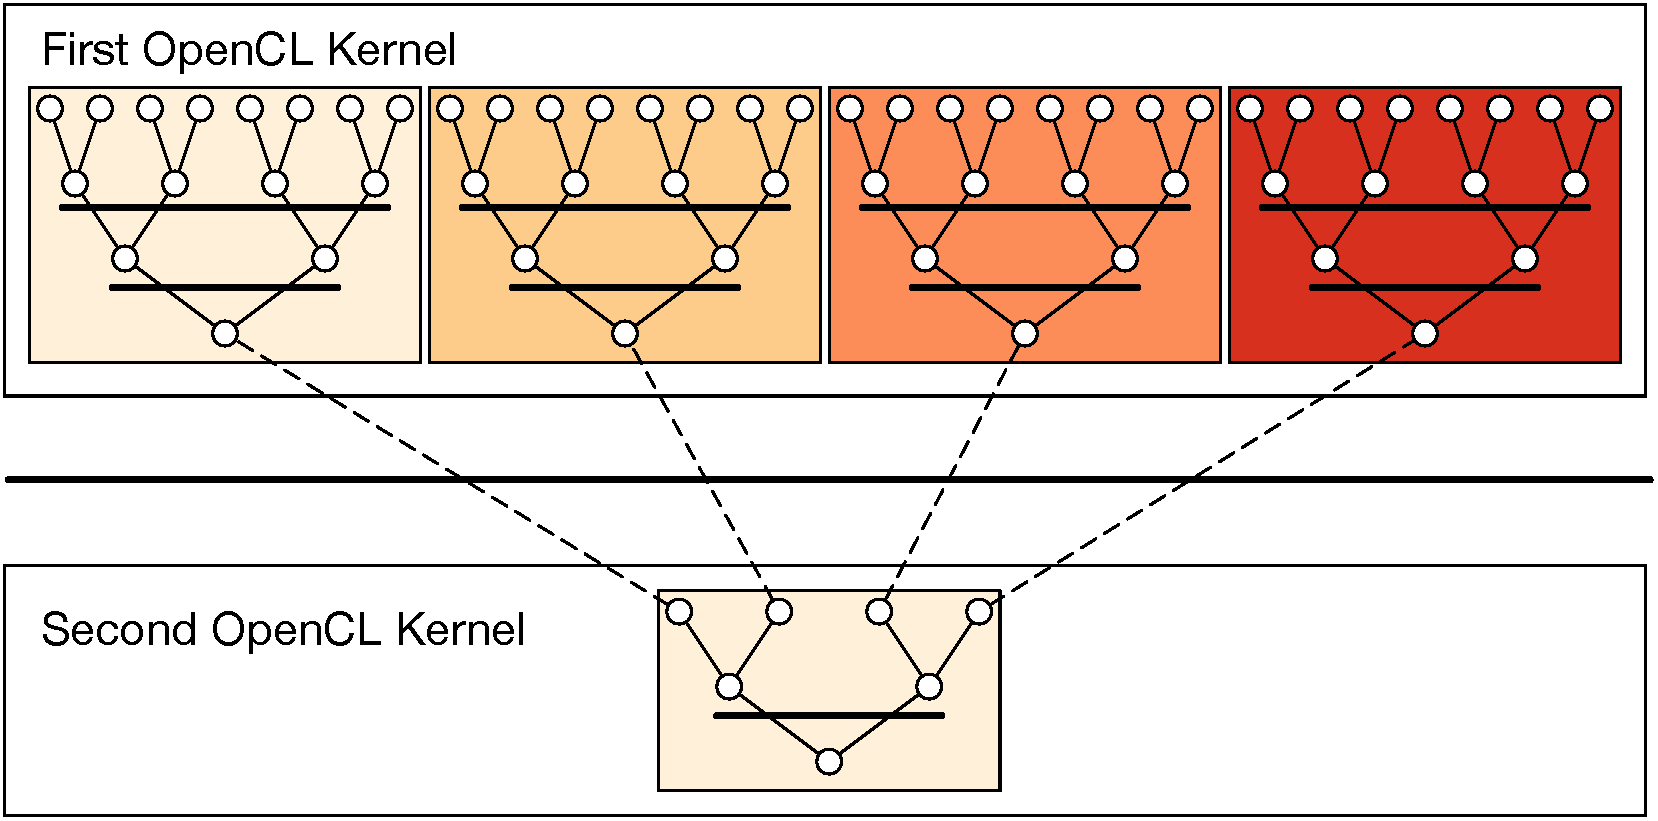
\includegraphics[width=.95\linewidth]{ReduceTree}
  \caption[Parallel Reduction in \OpenCL.]%
    {The first \OpenCL kernel is executed by four work-groups in parallel:
    \ \protect\firstBox{}\,\,work-group $0$,\ \protect\secondBox{}\,\,work-group $1$,\ \protect\thirdBox{}\,\,work-group $2$, \protect\fourthBox{}\,\,work-group $3$.
           The second \OpenCL kernel is only executed by the first work-group. The bold lines indicate synchronization points in the algorithm.}
  \label{fig:reduce:tree}
\end{figure}

We will follow the methodology established in~\cite{Harris2007} and evaluate the performance of the different versions using the measured \GPU memory bandwidth as our metric.
This is reasonable as the reduction has a very low arithmetic intensity and its performance is, therefore, bound by the available \GPU memory bandwidth.
By investigating the memory bandwidth of the \GPU memory, we can see which fraction of the maximum memory bandwidth available has been utilized.

All following implementations are provided by Nvidia as part of their software development kit and presented in~\cite{Harris2007}.
These implementations have originally been developed for Nvidia's Tesla \GPU architecture~\cite{LindholmNOM2008} and not been updated by Nvidia for more recent \GPU architectures.
Nevertheless, the optimizations discussed are still valid on more modern Nvidia \GPUs -- as we will see.
All performance numbers in this section have been measured on a Nvidia GTX 480 \GPU featuring the Nvidia Fermi architecture~\cite{CUDAFermi2009}.

\newpage

\paragraph{First \OpenCL implementation}
\autoref{lst:reduce0} shows the first version of the parallel reduction in \OpenCL.
%
\begin{lstlisting}[%
caption={[First \OpenCL implementation of the parallel reduction.]%
         First \OpenCL implementation of the parallel reduction achieving 6.64\% of the memory bandwith limit.},%
numbers=left,%
float=tb,
label={lst:reduce0}]
kernel
void reduce0(global float* g_idata, global float* g_odata,
             unsigned int n, local float* l_data) {
  unsigned int tid = get_local_id(0);
  unsigned int i   = get_global_id(0);
  l_data[tid] = (i < n) ? g_idata[i] : 0;$\label{lst:reduce0:load}$
  barrier(CLK_LOCAL_MEM_FENCE);$\label{lst:reduce0:firstBarrier}$
  // do reduction in local memory
  for(unsigned int s=1; s < get_local_size(0); s *= 2) {$\label{lst:reduce0:for:start}$
    if ((tid % (2*s)) == 0) {$\label{lst:reduce0:if}$
      l_data[tid] += l_data[tid + s]; }
    barrier(CLK_LOCAL_MEM_FENCE); }$\label{lst:reduce0:for:end}$
  // write result for this work-group to global memory
  if (tid == 0) g_odata[get_group_id(0)] = l_data[0]; }$\label{lst:reduce0:writeBack}$
\end{lstlisting}
% This will be our starting point for the following optimizations.
First each work-item loads an element into the local memory (\autoref{lst:reduce0:load}).
After a synchronization (\autoref{lst:reduce0:firstBarrier}) all work-items of a work-group execute a for loop (\autoref{lst:reduce0:for:start}---\autoref{lst:reduce0:for:end}) to perform a collective tree-based reduction.
In every iteration the if statement (\autoref{lst:reduce0:if}) ensures that a declining number of work-items remain active performing partial reductions in the shrinking reduction tree.
The second barrier in \autoref{lst:reduce0:for:end} ensures that no race conditions occur when accessing the shared local memory.
Finally, the work-item in the work-group with id $=0$ writes back the computed result to the global memory in \autoref{lst:reduce0:writeBack}.


The implementation presented in \autoref{lst:reduce0} is not straightforward to develop.
The application developer has to be familiar with the parallel execution model of \OpenCL to avoid race conditions and deadlocks.
For example, it is important that the second barrier in \autoref{lst:reduce0:for:end} is placed \emph{after} and not \emph{inside} the if statement.
This is true, even though work-items not entering the if statement will never read from or write to memory and, therefore, can never be influenced by a race condition.
Nevertheless, \OpenCL requires all work-items of a work-group to execute all barrier statements in a kernel exactly the same number of times.
The application developer is responsible to ensure that this condition is met, otherwise a deadlock will occur.

Despite being difficult to program, this implementation does not provide high performance either.
Only 6.64\% (11.78 GB/s) of the available bandwidth is utilized on the GTX 480.

\begin{lstlisting}[%
caption={[\OpenCL implementation of the parallel reduction avoiding divergent branching.]%
         \OpenCL implementation of the parallel reduction avoiding divergent branching.
         This implementation utilizes 9.73\% of the memory bandwidth limit.},%
numbers=left,%
float=tb,
label={lst:reduce1}]
kernel
void reduce1(global float* g_idata, global float* g_odata,
             unsigned int n, local float* l_data) {
  unsigned int tid = get_local_id(0);
  unsigned int i   = get_global_id(0);
  l_data[tid] = (i < n) ? g_idata[i] : 0;
  barrier(CLK_LOCAL_MEM_FENCE);

  for(unsigned int s=1; s < get_local_size(0); s *= 2) {
      // continuous work-items remain active
      $\strut$@int index = 2 * s * tid;@$\label{lst:reduce1:index}$
      if (@index < get_local_size(0)@) {$\label{lst:reduce1:if}$
          l_data[index] += l_data[index + s]; }$\label{lst:reduce1:read}$
      barrier(CLK_LOCAL_MEM_FENCE); }

  if (tid == 0) g_odata[get_group_id(0)] = l_data[0]; }
\end{lstlisting}

\paragraph{Avoid divergent branching}

\autoref{lst:reduce1} shows the second implementation.
The differences from the previous implementation are highlighted in the code.

When performing the collective tree-based reduction in a work-group, a shrinking number of work-items remain active until the last remaining work-item computes the result of the entire work-group.
In the previous version the modulo operator was used to determine which work-item remains active (see \autoref{lst:reduce0:if} in \autoref{lst:reduce0}).
This leads to a situation were not the consecutive work-items remain active, but rather work-items which id is divisible by 2, then by 4, then by 8, and so on.
In Nvidia's \GPU architectures, 32 work-items are grouped into a \emph{warp} and executed together, as described in \autoref{chapter:background}.
It is highly beneficial to program in a style where all 32 work-items grouped into a warp perform the same instructions to avoid divergent branching between work-items of a warp.
Using the modulo operator to determine the active work-items leads to highly divergent branching.
The second implementation in \autoref{lst:reduce1}, therefore, uses a different formula (\autoref{lst:reduce1:index}) for determining the active work-items, which avoids divergent branching.

The performance improves by a factor of 2.33 as compared to the first implementation.
However, still only 9.73\% (17.26 GB/s) of the theoretically available memory bandwidth are used by this version.


\FloatBarrier
\begin{lstlisting}[%
caption={[\OpenCL implementation of the parallel reduction avoiding local memory bank conflicts.]%
         \OpenCL implementation of the parallel reduction avoiding local memory bank conflicts.
         This implementation utilizes 12.61\% of the memory bandwidth limit.},%
numbers=left,%
float=tb,
label={lst:reduce2}]
kernel
void reduce2(global float* g_idata, global float* g_odata,
             unsigned int n, local float* l_data) {
  unsigned int tid = get_local_id(0);
  unsigned int i   = get_global_id(0);
  l_data[tid] = (i < n) ? g_idata[i] : 0;
  barrier(CLK_LOCAL_MEM_FENCE);

  // process elements in different order
  // requires commutativity!
  for(@unsigned int s=get_local_size(0)/2; s>0; s>>=1@) {$\label{lst:reduce2:s}$
      if (@tid < s@) {
          l_data[@tid@] += l_data[@tid@ + s]; }
      barrier(CLK_LOCAL_MEM_FENCE); }

  if (tid == 0) g_odata[get_group_id(0)] = l_data[0]; }
\end{lstlisting}

\paragraph{Avoid interleaved addressing}

\autoref{lst:reduce2} shows the third implementation.
The differences from the previous implementation are highlighted in the code.

On modern \GPUs the fast local memory is organized in multiple \emph{banks}.
When two, or more, work-items simultaneously access memory locations in the same bank a \emph{bank conflict} occurs which means that all memory requests are processed sequentially and not in parallel as usual.
The previous two implementations use an access pattern for the local memory which makes bank conflicts likely.
The third implementation in \autoref{lst:reduce2} avoids this problematic local memory access pattern.
Instead an access pattern is used where bank conflicts are unlikely and, thus, performance is improved.
This better access pattern requires the reduction operation to be commutative, as the order of element is not respected when reading from local memory.

The performance improves by a factor of 2.01 as compared to the previous implementation and 4.68 to the initial implementation.
With this version 12.61\% (22.37 GB/s) of the theoretically available memory bandwidth are used.



\FloatBarrier
\newpage

\paragraph{Increase computational intensity per work-item}

\autoref{lst:reduce3} shows the fourth implementation.
The differences from the previous implementation are highlighted in the code.
\begin{lstlisting}[%
caption={[\OpenCL implementation of the parallel reduction. Each work-item performs an addition when loading data from global memory.]%
         \OpenCL implementation of the parallel reduction. Each work-item performs an addition when loading data from global memory.
         This implementation utilizes 23.71\% of the memory bandwidth limit.},%
numbers=left,%
float=tb,
escapechar=\`,
label={lst:reduce3}]
kernel
void reduce3(global float* g_idata, global float* g_odata,
             unsigned int n, local float* l_data) {
  unsigned int tid = get_local_id(0);
  $\strut$@unsigned int i = get_group_id(0) * (get_local_size(0)*2)@
                                   $\strut$@+ get_local_id(0);@
  l_data[tid] = (i < n) ? g_idata[i] : 0;
  // performs first addition during loading
  $\strut$@if (i + get_local_size(0) < n)@
  $\strut$@    l_data[tid] += g_idata[i+get_local_size(0)];@$\label{lst:reduce3:comp}$
  barrier(CLK_LOCAL_MEM_FENCE);

  for(unsigned int s=get_local_size(0)/2; s>0; s>>=1) {
      if (tid < s) {
          l_data[tid] += l_data[tid + s]; }
      barrier(CLK_LOCAL_MEM_FENCE); }

  if (tid == 0) g_odata[get_group_id(0)] = l_data[0]; }
\end{lstlisting}

In the previous versions, each work-item loads one element from the global into the local memory before the work-items of the work-group collectively perform a tree-based reduction.
That means that half of the work-items are idle after performing a single copy operation, which is highly wasteful.
The fourth implementation in \autoref{lst:reduce3} avoids this by having each work-item load two elements from global memory, perform an addition, and store the computed result in local memory (\autoref{lst:reduce3:comp}).
Assuming the same input size this reduces the number of work-items to start with by half and, therefore, increases the computational intensity for every work-item.

The performance improves by a factor of 1.78 as compared to the previous implementation and 8.34 to the initial implementation.
With this version, 23.71\% (42.06 GB/s) of the theoretically available memory bandwidth is used.



\FloatBarrier
\newpage
\paragraph{Avoid synchronization inside a warp}

\autoref{lst:reduce4} shows the fifth implementation.
The differences from the previous implementation are highlighted in the code.

Wraps are the fundamental execution unit in Nvidia's \GPU architectures, as explained in \autoref{chapter:background}:
32 work-items are grouped together to form a warp based on their id, \ie, work-items with id $0$ -- 31 are grouped into the first warp, work-items with id 32 -- 63 into the second warp, and so on.
All work-items grouped in a warp are guaranteed to be executed together in a lock-step manner, \ie, all work-items in the same warp execute the same instruction simultaneously.
Because of this hardware behaviour, no barrier synchronization is required between instructions inside a single warp.
The fifth implementation in \autoref{lst:reduce4} takes advantage of this.
The for loop performing the tree-based reduction is exited early at the stage when only 32 work-items remain active (see \autoref{lst:reduce4:for}).
The extra code in \autoref{lst:reduce4:warp:start} up to \autoref{lst:reduce4:warp:end} performs the rest of the tree-base reduction without any barrier synchronization.
The code shown here effectively unrolled the last six iterations of the for loop in \autoref{lst:reduce4:for}.
As warps are specific to Nvidia's \GPU architectures, this implementation is not portable and might produce incorrect results on other \OpenCL devices.

The performance improves by a factor of 1.8 as compared to the previous implementation and 15.01 to the initial implementation.
With this version, 32.59\% (57.81 GB/s) of the theoretically available memory bandwidth is used.

\begin{lstlisting}[%
caption={
         [\OpenCL implementation of the parallel reduction.
         Synchronization inside a warp is avoided by unrolling the loop for the last 32 work-items.]
         \OpenCL implementation of the parallel reduction.
         Synchronization inside a warp is avoided by unrolling the loop for the last 32 work-items.
         This implementation utilizes 32.59\% of the memory bandwidth limit.},%
numbers=left,%
float=p,
label={lst:reduce4}]
kernel
void reduce4(global float* g_idata, global float* g_odata,
             unsigned int n,local volatile float* l_data){
  unsigned int tid = get_local_id(0);
  unsigned int i = get_group_id(0) * (get_local_size(0)*2)
                                   + get_local_id(0);
  l_data[tid] = (i < n) ? g_idata[i] : 0;
  if (i + get_local_size(0) < n)
      l_data[tid] += g_idata[i+get_local_size(0)];
  barrier(CLK_LOCAL_MEM_FENCE);

  // prevent further unrolling (see next version)
  $\strut$@#pragma unroll 1@$\label{lst:reduce4:pragma}$
  for(unsigned int s=get_local_size(0)/2; s>@32@; s>>=1) {$\label{lst:reduce4:for}$
      if (tid < s) {
          l_data[tid] += l_data[tid + s]; }
      barrier(CLK_LOCAL_MEM_FENCE); }

  // unroll for last 32 active work-items
  // no synchronization required on NVIDIA GPUs
  // this is not protable OpenCL code!
  $\strut$@if (tid < 32) {@$\label{lst:reduce4:warp:start}$
  $\strut$@  if (WG_SIZE >= 64) { l_data[tid] += l_data[tid+32]; }@
  $\strut$@  if (WG_SIZE >= 32) { l_data[tid] += l_data[tid+16]; }@
  $\strut$@  if (WG_SIZE >= 16) { l_data[tid] += l_data[tid+ 8]; }@
  $\strut$@  if (WG_SIZE >=  8) { l_data[tid] += l_data[tid+ 4]; }@
  $\strut$@  if (WG_SIZE >=  4) { l_data[tid] += l_data[tid+ 2]; }@
  $\strut$@  if (WG_SIZE >=  2) { l_data[tid] += l_data[tid+ 1]; } }@$\label{lst:reduce4:warp:end}$

  if (tid == 0) g_odata[get_group_id(0)] = l_data[0]; }
\end{lstlisting}

\paragraph{Complete loop unrolling}

\autoref{lst:reduce5} on page~\pageref{lst:reduce5} shows the sixth implementation.
The differences from the previous implementation are highlighted in the code.

In the previous implementation we made a special case for the last six iterations of the for loop and provided special code handling for each iteration separately.
This is a general optimization strategy known as \emph{loop unrolling}.
Loop unrolling can be beneficial because variables and branches required by a loop can be avoided.
Furthermore, instruction level parallelism can be increased.
In the sixth implementation, shown in \autoref{lst:reduce5}, the for loop has been removed entirely and replaced by three if statement (\autoref{lst:reduce5:if:1}, \autoref{lst:reduce5:if:2}, and \autoref{lst:reduce5:if:3}).
Each if statement replaces one iteration of the loop.
This code assumes that \code{WG\_SIZE} is a compile-time constant and, therefore, the if statements will be evaluated at compile time, avoiding costly branches at runtime.
Different to the previous optimization (\autoref{lst:reduce4}), we still have to provide a barrier to ensure correct synchronization, as multiple warps are involved here.

The performance improves by a factor of 1.41 as compared to the previous implementation and 21.16 times as compared to the initial implementation.
With this version, 36.77\% (65.23 GB/s) of the theoretically available memory bandwidth are used.

\begin{lstlisting}[%
caption={[\OpenCL implementation of the parallel reduction with a completly unrolled loop.]
         \OpenCL implementation of the parallel reduction with a completly unrolled loop.
         This implementation utilizes 36.77\% of the memory bandwidth limit.},%
numbers=left,%
float=p,
label={lst:reduce5}]
kernel
void reduce5(global float* g_idata, global float* g_odata,
             unsigned int n,local volatile float* l_data){
  unsigned int tid = get_local_id(0);
  unsigned int i = get_group_id(0) * (get_local_size(0)*2)
                                   + get_local_id(0);
  l_data[tid] = (i < n) ? g_idata[i] : 0;
  if (i + get_local_size(0) < n)
      l_data[tid] += g_idata[i+get_local_size(0)];
  barrier(CLK_LOCAL_MEM_FENCE);

  // unroll for loop entirely
  $\strut$@if (WG_SIZE >= 512) {@$\label{lst:reduce5:if:1}$
  $\strut$@    if (tid < 256) { l_data[tid] += l_data[tid+256]; }@
  $\strut$@    barrier(CLK_LOCAL_MEM_FENCE); }@
  $\strut$@if (WG_SIZE >= 256) {@$\label{lst:reduce5:if:2}$
  $\strut$@    if (tid < 128) { l_data[tid] += l_data[tid+128]; }@
  $\strut$@    barrier(CLK_LOCAL_MEM_FENCE); }@
  $\strut$@if (WG_SIZE >= 128) {@$\label{lst:reduce5:if:3}$
  $\strut$@    if (tid <  64) { l_data[tid] += l_data[tid+ 64]; }@
  $\strut$@    barrier(CLK_LOCAL_MEM_FENCE); }@

  if (tid < 32) {
    if (WG_SIZE >= 64) { l_data[tid] += l_data[tid+32]; }
    if (WG_SIZE >= 32) { l_data[tid] += l_data[tid+16]; }
    if (WG_SIZE >= 16) { l_data[tid] += l_data[tid+ 8]; }
    if (WG_SIZE >=  8) { l_data[tid] += l_data[tid+ 4]; }
    if (WG_SIZE >=  4) { l_data[tid] += l_data[tid+ 2]; }
    if (WG_SIZE >=  2) { l_data[tid] += l_data[tid+ 1]; } }

  if (tid == 0) g_odata[get_group_id(0)] = l_data[0]; }
\end{lstlisting}


\paragraph{Fully optimized implementation\hfill\strut}

\autoref{lst:reduce6} on page~\pageref{lst:reduce6} shows the final and fully optimized implementation.
The differences from the previous implementation are highlighted in the code.

One of the optimizations applied earlier was to increase the computational intensity for each single work-item by performing two loads and an addition instead of a single load.
This final version applies the same idea, but performing multiple additions per work-item before the collective tree-based reduction in the entire work-group.
This has indeed two advantages:
first, the algorithmic intensity is increased, \ie, each work-item is doing more work,
and, second, performing the summation sequentially by a single work-item does not require costly synchronizations.
The fully optimized implementation is shown in \autoref{lst:reduce6} with the changes highlighted.
A while loop has been introduced (see \autoref{lst:reduce6:while}) which, in every iteration, loads two elements from the global memory and adds them to the local memory.
No synchronization is required here as each work-item operates independently on different memory locations.
The way the memory is accessed ensures that memory accesses will be coalesced (see \autoref{chapter:background}) when reading from global memory.

The performance improves by a factor of 1.42 as compared to the previous implementation and 30.04 times as compared to the initial implementation.
With this version, 65.44\% (116.09 GB/s) of the theoretically available memory bandwidth are used.

\begin{lstlisting}[%
caption={[Fully optimized \OpenCL implementation of the parallel reduction.]
         Fully optimized \OpenCL implementation of the parallel reduction.
         This implementation utilizes 65.44\% of the memory bandwidth limit.},%
numbers=left,%
float=p,
label={lst:reduce6}]
kernel
void reduce6(global float* g_idata, global float* g_odata,
             unsigned int n,local volatile float* l_data){
  unsigned int tid = get_local_id(0);
  unsigned int i = get_group_id(0) * (get_local_size(0)*2)
                                   + get_local_id(0);
  $\strut$@unsigned int gridSize = WG_SIZE*2*get_num_groups(0);@
  $\strut$@l_data[tid] = 0;@

  // multiple elements are reduced per work-item
  $\strut$@while (i < n) { l_data[tid] += g_idata[i];@$\label{lst:reduce6:while}$
  $\strut$@                if (i + WG_SIZE < n)@
  $\strut$@                  l_data[tid] += g_idata[i+WG_SIZE];@
  $\strut$@                i += gridSize; }@
  barrier(CLK_LOCAL_MEM_FENCE);

  if (WG_SIZE >= 512) {
      if (tid < 256) { l_data[tid] += l_data[tid+256]; }
      barrier(CLK_LOCAL_MEM_FENCE); }
  if (WG_SIZE >= 256) {
      if (tid < 128) { l_data[tid] += l_data[tid+128]; }
      barrier(CLK_LOCAL_MEM_FENCE); }
  if (WG_SIZE >= 128) {
      if (tid <  64) { l_data[tid] += l_data[tid+ 64]; }
      barrier(CLK_LOCAL_MEM_FENCE); }

  if (tid < 32) {
    if (WG_SIZE >= 64) { l_data[tid] += l_data[tid+32]; }
    if (WG_SIZE >= 32) { l_data[tid] += l_data[tid+16]; }
    if (WG_SIZE >= 16) { l_data[tid] += l_data[tid+ 8]; }
    if (WG_SIZE >=  8) { l_data[tid] += l_data[tid+ 4]; }
    if (WG_SIZE >=  4) { l_data[tid] += l_data[tid+ 2]; }
    if (WG_SIZE >=  2) { l_data[tid] += l_data[tid+ 1]; } }

  if (tid == 0) g_odata[get_group_id(0)] = l_data[0]; }
\end{lstlisting}


\paragraph{Conclusions\hfill\strut}
We can draw several valuable conclusions from studying these \OpenCL source codes.

The first main conclusion is, that implementing these optimizations is not intuitive and straightforward.
It requires experience as well as knowledge and reasoning about the target hardware architecture, in this case the Fermi \GPU architecture:
\autoref{lst:reduce1} requires the understanding of the problem of \emph{branch divergence}, \autoref{lst:reduce2} requires knowledge about the organization of local memory and \emph{bank conflicts}, \autoref{lst:reduce3} and \autoref{lst:reduce6} require reasoning about the \emph{computational intensity} of work-items, \autoref{lst:reduce4} requires understanding of \emph{warps} and their execution by the hardware, \autoref{lst:reduce5} requires experience with \emph{loop unrolling} techniques, and, finally, \autoref{lst:reduce6} required knowledge about the organization of global memory and \emph{memory coalescing}.
The author wants to empathize that these are \emph{additional} burdens for the application developer on top of implementing a functionally correct version where the programmer is facing widely recognized correctness problems of parallel programming like race conditions and deadlocks.

Furthermore, the source code changes necessary for individual optimization steps are not obvious either.
While the performance increases gradually, the source code changes are more radical.
The source code of the first implementation in \autoref{lst:reduce0} is very different as compared to the final implementation shown in \autoref{lst:reduce6}.
For example, the code size has more then doubled (from 16 to 35 lines of code) and many statements have been added or replaced others.
It is not obvious, neither to a human being nor to an optimizing compiler, that these two pieces of code have the same semantics (assuming an associative and commutative binary reduction operator, like $+$).

The second main conclusion we can draw is, that performing these optimizations on modern parallel architectures is highly beneficial.
The first unoptimized version did only utilize about 6.64\% of the available memory bandwidth, while the fully optimized version utilizes a more reasonable 65.44\% on our GeForce GTX 480.
Applying all optimizations improved the performance by a factor of $\approx${}$10$ while utilizing the exactly same hardware.
For an input array of size of 256 MB the runtime reduces from 95.7 ms to 9.1 ms when using the optimized kernel over the unoptimized one.
Harris~\cite{Harris2007} reports an even higher improvement factor of $\approx${}$30$ for the GeForce 8800 GTX used in his experiments.
Modern parallel processors are often chosen as target architecture because of their high theoretical performance.
Turning the theoretical performance into practical performance by applying such optimizations is, therefore, \emph{essential} for most users.





\subsection{Portability of the Optimized Parallel Reduction}
After we have established how crucial but hard to achieve optimizations are, we now will investigate their portability.
To do so, we did run the code shown in \autoref{lst:reduce0}--\autoref{lst:reduce6} on three different hardware devices:
Nvidia's GTX 480 (Fermi \GPU architecture~\cite{CUDAFermi2009}) which we have used in our analysis in the previous section, AMD's Radeon HD7970 (Graphics Core Next \GPU architecture~\cite{AMDGCN2012}), and Intel's E5530 \CPU (Nehalem \CPU architecture~\cite{IntelNehalem2008}).
\autoref{fig:reduce:overview} shows the performance numbers for each device.
We use, as before, the memory bandwidth as our performance metric and show the hardware memory bandwidth limit of each respective hardware architecture at the top.
As a practical comparison we also show performance numbers for the parallel reduction using highly tuned, architecture specific implementations of the BLAS library.
We use the CUBLAS library~\cite{cuBLAS} for the Nvidia \GPU, the clBLAS library~\cite{clBLAS} for the AMD \GPU, and the MKL library~\cite{MKL} for the Intel \CPU.
Each library is implemented and provided by the corresponding hardware vendor.

\begin{figure}[p]
  \centering
\begin{subfigure}{\linewidth}
  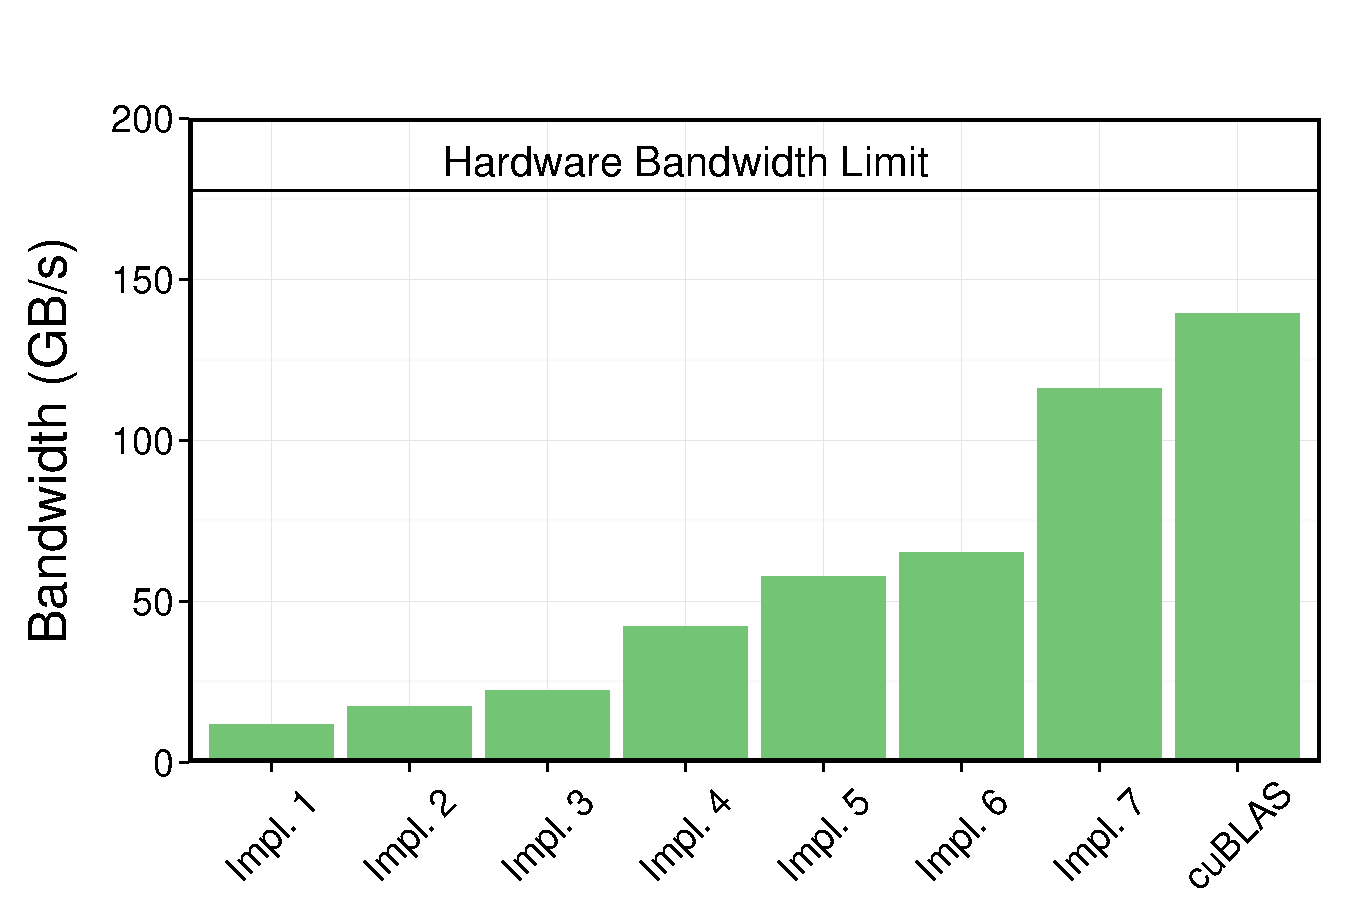
\includegraphics[width=.85\linewidth]{Plots/Reduction/reduce_nv}
  \caption{Nvidia's GTX 480 \GPU.}
  \label{fig:reduce:nvidia}
\end{subfigure}\\
\begin{subfigure}{\linewidth}
  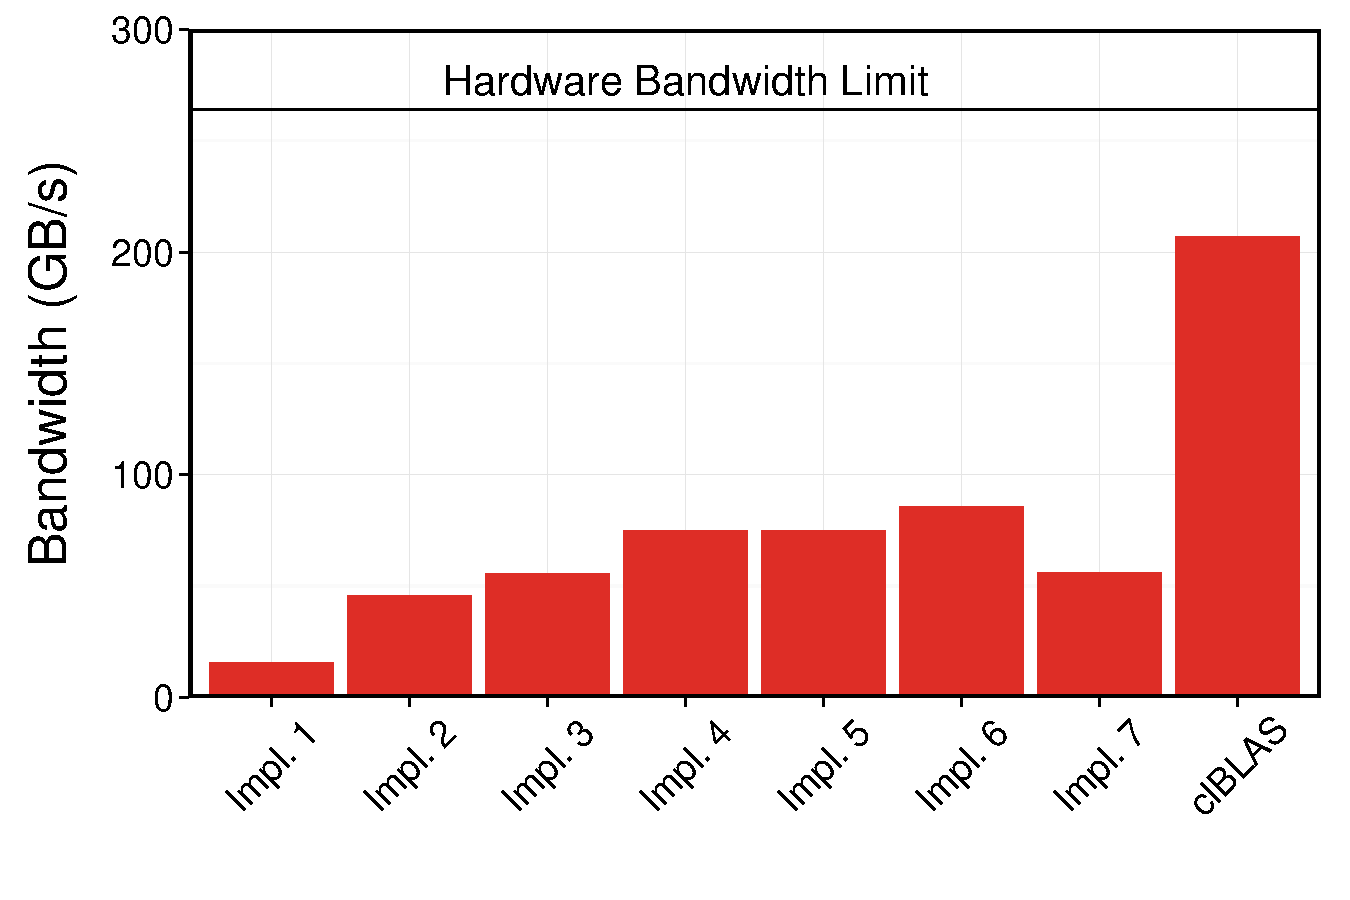
\includegraphics[width=.85\linewidth]{Plots/Reduction/reduce_amd}
  \caption{AMD's HD 7970 \GPU.}
  \label{fig:reduce:amd}
\end{subfigure}\\
\begin{subfigure}{\linewidth}
  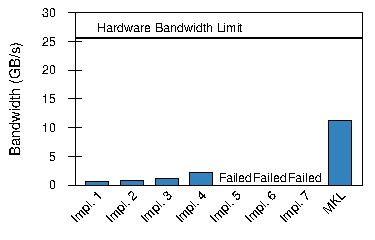
\includegraphics[width=.85\linewidth]{Plots/Reduction/reduce_intel}
    \caption{Intel's E5530 dual-socket \CPU.}
  \label{fig:reduce:intel}
\end{subfigure}
  \caption[Performance of optimized implementations of the parallel reduction]{Performance of differently optimized implementations of the parallel reduction}
  \label{fig:reduce:overview}
\end{figure}


\paragraph{Portability of Optimizations}
The results show that the optimizations discussed in the previous section are not portable.
On each architecture a different version of the optimized implementations performs best:
Implementation~7 (shown in \autoref{lst:reduce6}) on the Nvidia \GPU, Implementation~6 (shown in \autoref{lst:reduce5}) on the AMD \GPU, and Implementation~4 (shown in \autoref{lst:reduce3}) on the Intel \CPU.
Some implementations actually produce incorrect results on the Intel \CPU due to the warp-specific optimization introduced in Implementation~5 (shown in \autoref{lst:reduce4}).
Interestingly, this optimization happens to be valid on AMD's \GPU architecture as well, as there exists a similar concept to warps called \emph{wavefronts}~\cite{AMDGCN2012}.

\paragraph{Portability of Relative Performance}
\emph{Relative performance} refers to the performance of an implementation relative to the best theoretical or practical performance possible on a given hardware architecture.
The theoretical performance of an architecture is given by its hardware limitations, like the number of arithmetic logical units, the width of the memory bus, or the maximum clock frequency.
Practical issues like work load and utilization or the cache miss rate are ignored.
Possible metrics for measuring the theoretical performance are number of floating point operation in GFLOP/s or the memory bandwidth in GB/s.

The best practical performance is measured by comparison with the best possible implementation available for a particular hardware platform.
It is not always possible to determine which implementation is the best.
Here we consider the BLAS library implementations tuned by the respective hardware vendors as the best available.

By investigating relative performance we can compare how well optimizations apply across different hardware architectures.
The \emph{relative performance} shown in \autoref{fig:reduce:overview} differs widely across architectures. %, as we can see in \autoref{fig:reduce:overview}.

On the Nvidia \GPU, the best optimized implementation achieves 83.3\% of the performance of the vendor-provided CUBLAS implementation utilizing 65.4\% of the theoretical memory bandwidth limit.

On the AMD \GPU, the gap between the manual and library implementation is much larger:
the manually optimized implementation achieves only 41.3\% of the clBLAS library implementation.
Only 32.4\% of the theoretical memory bandwidth limit is achieved.

On the Intel \CPU, implementation~4 achieves only 16.6\% of the MKL performance.
That means, that MKL is over 5 times faster than the best of the discussed implementations.
The hardware bandwidth limit is only utilized to 8.6\%.
Interestingly, the MKL implementation also only provides 43.8\% of the maximum memory bandwidth.
This is due to the combination of the implementation of the parallel reduction in MKL and the particular machine used in this experiment.
The test machine used is configured as a dual-socket machine, \ie, two E5530 \CPUs each with their own memory controller are available.
Therefore, the hardware bandwidth available is doubled as compared to a single E5530 \CPU.
While the implementation of the parallel reduction in the MKL library is optimized using vector instructions, it does not exploit thread-level parallelism.
Therefore, the second E5530 \CPU can not be used by the implementation, thus, limiting the available bandwidth by half.

\paragraph{Conclusions}
Studying the performance of the optimizations presented by Harris~\cite{Harris2007} on different hardware architectures gained some interesting insides.
First, optimizations are not portable across hardware architectures and can even result in incorrect programs on some architectures.
Second, the relative performance achieved with optimizations on one architecture is not always achieved on other hardware architectures as well.
This let us conclude that performance is \emph{not} portable when using \OpenCL or similar low-level approaches.

As a positive result we can see from \autoref{fig:reduce:overview} that there exist implementations on the other hardware architectures which offer similar relative performance as the most optimized implementation on the Nvidia \GPU.
For the AMD \GPU, the clBLAS implementation achieves 78.5\% of the hardware bandwidth limit and Intel's MKL implementation achieves 87.6\% of the hardware limit, considering just the bandwidth of a single \CPU socket.

We aim at developing an approach which can systematically apply optimizations and generate code matching the performance on all three architectures, thus, offering performance portability.

% In the following we aim for developing an approach where we can systematically describe and apply optimizations to eventually automatically generate highly efficient, hardware specific code.
% This will ultimately lead to performance portable code.

%\todo{This approach should be able to apply all optimizations we just discussed ...}

\subsection{The Need for a Pattern-Based Code Generator}

Our main goal in this chapter is to develop a systematic approach to achieve \emph{performance portability}, \ie, to achieve high relative performance for a given application across a set of different parallel processors.
As we saw in the previous section, traditional approaches, like \OpenCL, are not performance portable.
Currently, programmers often tune their implementations towards a particular hardware using hardware-specific optimizations to achieve the highest performance possible, as seen in \autoref{lst:reduce4}.
This reduces portability, maintainability, and clarity of the code:
multiple versions have to be maintained, and non-obvious optimizations make the code hard to understand and to reason about.

We argue that \emph{parallel patterns} can help overcome the tension between achieving the highest possible performance and preserving code portability and maintainability.
Parallel patterns declaratively specify the desired algorithmic behavior, rather than encode a particular implementation which might offer suboptimal performance on some hardware architectures.
A parallel pattern can be implemented in different ways, optimized towards particular hardware architectures.
If the underlying hardware is changed, the optimal implementation for the new hardware can be chosen.

While a compelling idea in theory, existing approaches have fallen short of providing and selecting highly optimized implementations on different architectures.
Previous work has been limited to ad-hoc solutions for specific hardware architectures.
This limitation has three main reasons:

First, providing optimized implementations of pattern on every new hardware platform is a challenging task.
Nowadays, dozens of parallel architectures and hundreds of variations of them exist and new architectures are released every year.
Therefore, it is often not feasible to provide optimized implementations for all available hardware architectures and existing library approaches have focused on particular hardware architectures.
For example, Nvidia \GPUs have been the main target for the \SkelCL library and, therefore, the skeleton implementations have been optimized appropriately.
The \stencil skeleton implementation, for example, makes heavy use of the local memory feature of \OpenCL which is usually not beneficial to be used on a \CPU, as \CPUs do not feature the corresponding memory area in hardware.
An approach using code generation could overcome this drawback, because instead of fixed implementations collected in a library rather possible optimizations are systematically described and then automatically applied by the code generator.

\bigskip

Second, most existing approaches are library-based, which makes the optimization of composition and nesting of patterns extremely complex.
In \SkelCL, for example, each pattern is implemented as a separate \OpenCL kernel.
When composing patterns, multiple kernels are executed, but often a better solution would be to fuse multiple kernels into a single kernel, thus avoiding costly operations to write and read the intermediate result into/from the global memory.
As fusion of \OpenCL kernels in general is complicated and requires code analysis, \SkelCL currently cannot execute a fused, and, thus, fully optimized, implementation of composed patterns.
Our envisaged approach using code generation should overcome this issue, as the code generator processes the entire pattern-based expression instead of focusing on individual patterns.

\bigskip

Finally, the optimal implementation of a parallel pattern usually depends very much on the application and context the pattern is used in.
For example, the algorithmic skeleton \reduce can be used on its own to implement a parallel summation, as discussed in \autoref{sec:reduce:case-study}, but it can also be used as part of the dot product computation which itself is a building block of matrix multiplication, as we saw in \autoref{chapter:skelcl}.
The optimal implementation of \reduce will most certainly differ across these use cases.
Indeed, for the parallel summation the entire parallel processor should be exploited using many \OpenCL work-items simultaneously, while when being executed as part of the matrix multiplication \reduce should only exploit thread level parallelism to a limited degree -- if at all.
An approach using code generation could overcome this issue, as specialized code can be generated for patterns in different contexts instead of providing a single fixed implementation.

\clearpage

% what is our approach
We argue that the root of the problem lies in a gap in the system stack between the high-level algorithmic patterns on the one hand and low-level hardware optimizations on the other hand.
We propose to bridge this gap using a novel pattern-based code generation technique.
A set of rewrite rules systematically translates high-level algorithmic patterns into low-level hardware patterns.
The rewrite rules express different algorithmic and optimization choices.
By systematically applying the rewrite rules semantically equivalent, low-level expressions are derived from high-level algorithm expressions written by the application developer.
Once derived, high-performance code based on these expressions can be automatically generated.
The next section introduces an overview of our approach.

